\newchapter{phasePropagation}{Phase Propagation}

This is the introductory text.

\newsection{origJitter}{Characteristics of Uncorrected Phase Jitter}

Injector feedbacks etc.

Definitions of different types of phase jitter.

\newsection{r56}{First Order Energy Dependencies}

\subsection{Correlation between Phase and Energy}
\label{ss:corrPhaseEnergy}

\subsection{Expected Dependence due to Optics}
\label{ss:r56Sim}

\begin{figure}
  \centering
  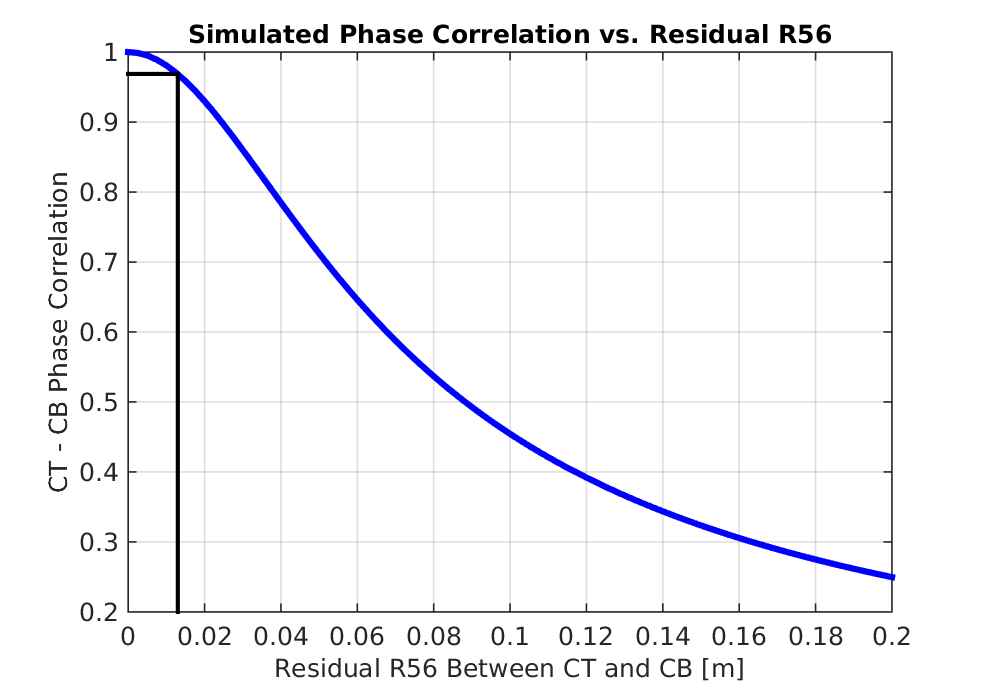
\includegraphics[width=0.45\textwidth]{Figures/R56_corrSim}
  \caption{Phase correlation vs. residual R56 between monitors.}
  \label{f:R56_corrSim}
\end{figure}

\newsection{r56Removal}{Mitigation of First Order Energy Dependence}

\subsection{TL1}
\label{ss:tl1}

\subsection{Matched Optics for TL1}
\label{ss:tl1Optics}

\subsection{Scans of R56 in TL1}
\label{ss:r56Scans}

\newsection{t566}{Higher Order Energy Dependencies}

\subsection{Expected Dependence due to Optics}
\label{ss:t566Sim}

\subsection{Energy Variation Along the Pulse}
\label{ss:energyAlongPulse}

\subsection{R56 Scans whilst Varying Beam Energy}
\label{ss:r56ScanWithEnergy}

\begin{figure}
  \centering
  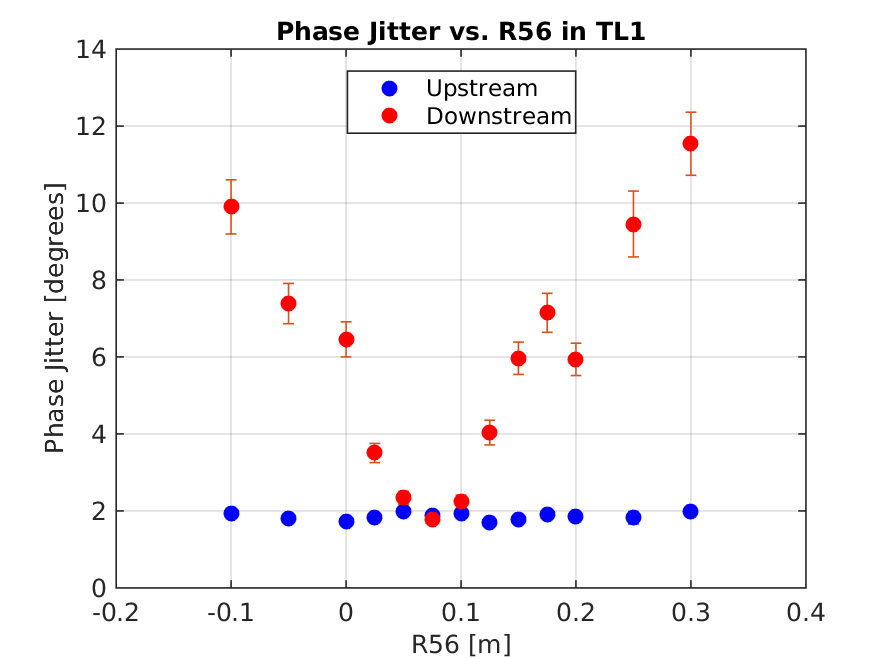
\includegraphics[width=0.45\textwidth]{Figures/R56ScanGunWiggle_PhaseJitter}
  \caption{Phase jitter for different R56 whilst wiggling gun current.}
  \label{f:R56ScanGunWiggle_PhaseJitter}
\end{figure}

\begin{figure}
  \centering
  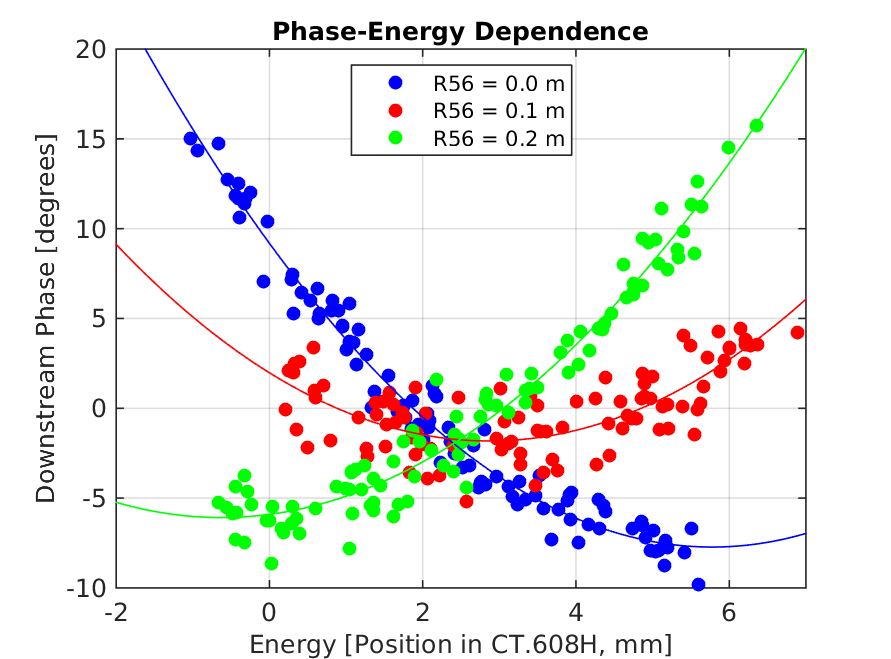
\includegraphics[width=0.45\textwidth]{Figures/R56ScanGunWiggle_Vs608}
  \caption{Phase vs. energy for different R56 in TL1.}
  \label{f:R56ScanGunWiggle_Vs608}
\end{figure}

\subsection{Effect on PFF Operation}
\label{ss:t566EffectPFF}


\newsection{otherJitterSources}{Other Sources of Phase Jitter}

\subsection{Combiner Ring Septum}
\label{ss:crSeptum}

\subsection{TL1 \& Combiner Ring Bends}
\label{ss:crBends}


RF Deflector

CR Septum

TL1/CR Bends


\newsection{longTermStability}{Long Term Propagation Stability}





